\Section{$\alpha$ Plot}
%\label{$\alpha$ plot}
We have shown $\alpha$ for three kinematic settings in \Tableref{alpha1} plotted in BLUE in \figureref{alpha} with respect to hydrogen target. The available $\alpha$ values from proton and pion analysis have been shown in RED and GREEN, respectively, for comparison. We considered only the statistical uncertainties which are shown by closed vertical lines. The experimental $\alpha$ values from the processes other than electro-production are shown by the horizontal band in \figureref{alpha}. The width of the band represents statistical uncertainty.

\begin{figure}[!tbp]
  \centering
  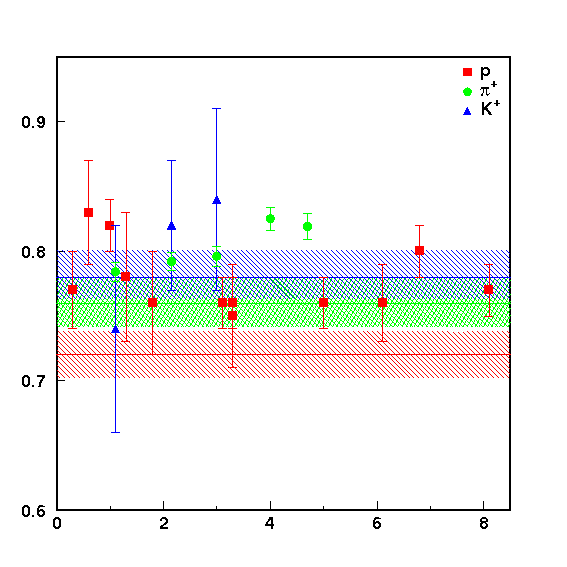
\includegraphics[trim = 8mm 8mm 8mm 8mm, clip,width=0.8\columnwidth]{alpha}
  \caption[$\alpha$ for different kinematics electro-production and hadro-production.]{\label{fig:alpha}$\alpha$ for different kinematics electro-production and hadro-production.\\\\ Electro-production data points in RED are for protons, GREEN data points are for $\pi^+$ and BLUE data points are from this analysis for $K^+$. Similarly, horizontal lines corresponds to $\alpha$ values from hadron-scattering with error band for different hadrons.}
\end{figure}
%\Figure{alpha}{\figwidth}{$\alpha$ for different kinematics electro-production and hadro-production. Electro-production data points in \textcolor{red}{RED} are for protons, \textcolor{green}{GREEN} data points are for $\pi^+$ and \textcolor{blue}{BLUE} data points are from this analysis for $K^+$. Similarly, horizontal lines corresponds to $\alpha$ values from hadron-scattering with error band for different hadrons.}
\begin{table}
  \caption{$\alpha$ values for different $Q^2$ for kaons with respect to hydrogen.}
  \label{tab:alpha1}
\begin{center}
\begin{tabular}{||c|c|c||}\hline
 Kinematics & $Q^2$ & $\alpha$ \\
 & $(GeV/c)^2$ & \\\hline
Kin1 & 1.1 &0.84$\pm$0.06 \\
Kin2 & 2.2 &0.91$\pm$0.04 \\
Kin3 & 3.0 &0.92$\pm$0.05 \\\hline
\end{tabular}
\vspace{-0.5cm}
\end{center}
\end{table}
%\Table{alpha1}{$\alpha$ values for different $Q^2$ for kaons with respect to hydrogen.}
\newpage
\Section{Comparison of Yields for Data with SIMC}
We already discussed in section \ref{Comparison of Data with SIMC Yields} about the dependency of the cross section upon four variables: $Q^2$, $W$, $t$ and $\phi_{pq}$, where $Q^2$ is four-momentum transferred square, $W$ is the center of mass energy, $t$ is momentum transfer, and $\phi_{pq}$ is  the angle between the scattering and reaction planes. In this appendix, we are showing comparison of SIMC and data yields for missing mass, $W$, $t$ and $\phi_{pq}$ in the \figureref{missmass2}, \figureref{com_plot_w_2}, \figureref{com_plot_t_2} and \figureref{com_plot_phi_2}, respectively. We have already shown the comparison for $Q^2$ in section \ref{Comparison of Data with SIMC Yields}.

\begin{figure}[!tbp]
  \centering
  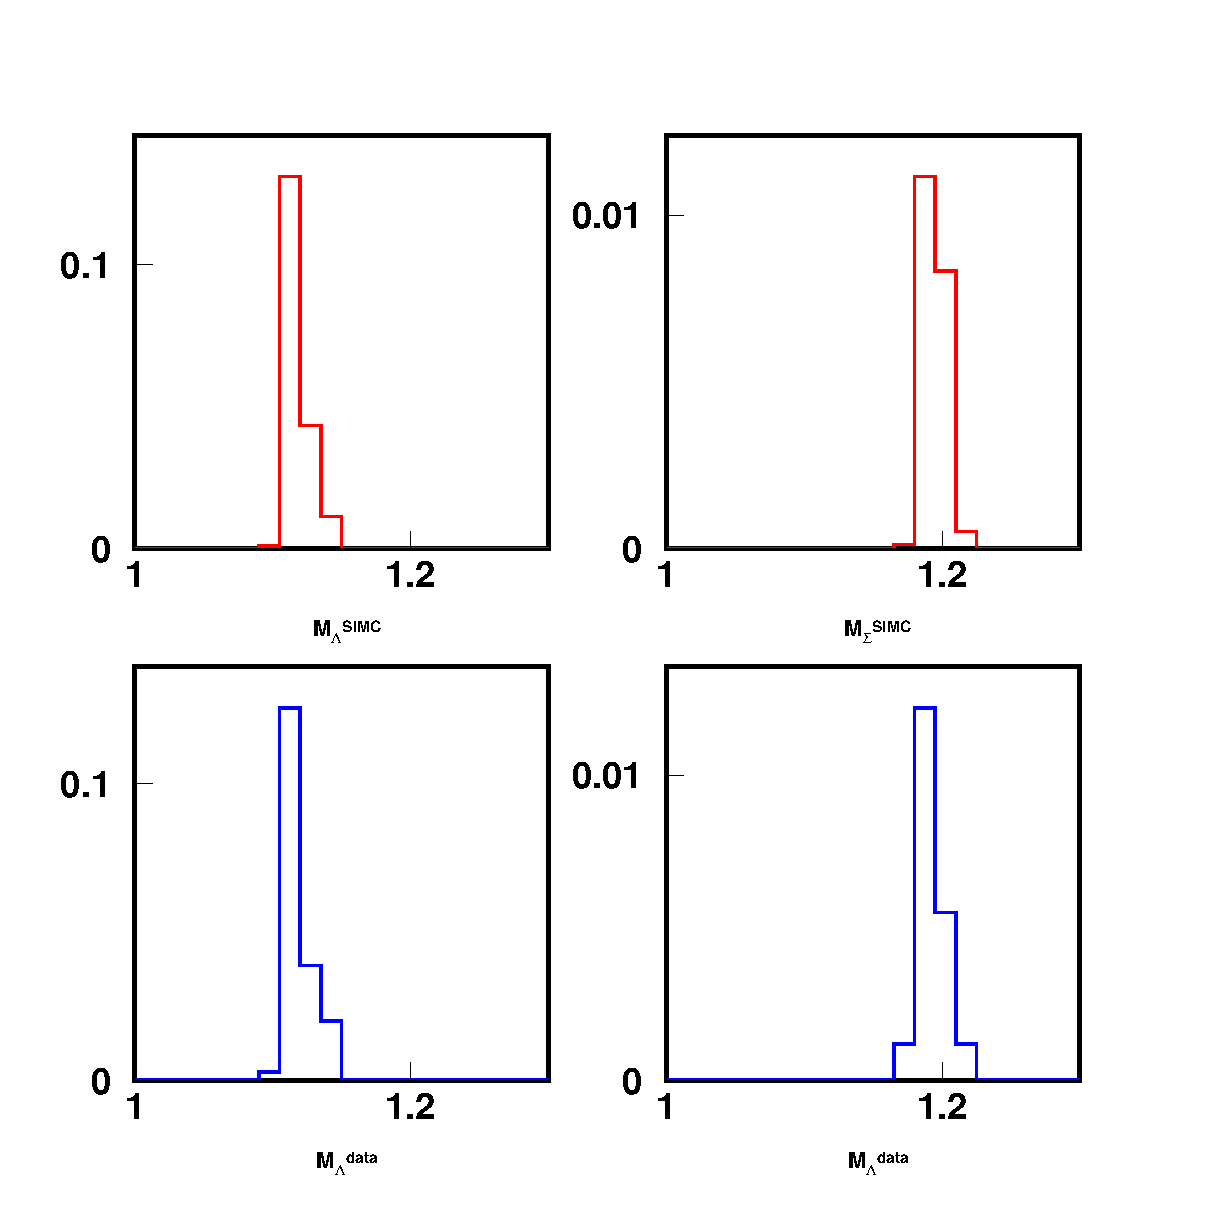
\includegraphics[width=0.8\columnwidth]{missmass2}
  \caption[Missing mass are shown here after applying cuts.]{\label{fig:missmass2}Missing mass are shown here after applying cuts.\\\\ One-dimensional plot of missing mass are shown here after applying all the cuts. Clockwise top left corner: $M_\Lambda^{SIMC}$ and $M_\Sigma^{SIMC}$ in RED, $M_\Sigma^{data}$ and $M_\Lambda^{data}$ in BLUE for $Q^2$=2.2 $(\mathrm{GeV/c})^2$.}
\end{figure}
%\Figure{missmass2}{\figwidth}{One-dimensional plot of missing mass are shown here after applying cuts. Clockwise top left corner: $M_\Lambda^{SIMC}$ and $M_\Sigma^{SIMC}$ in \textcolor{red}{RED}, $M_\Sigma^{data}$ and $M_\Lambda^{data}$ in \textcolor{blue}{BLUE}.}

\begin{figure}[!tbp]
  \centering
  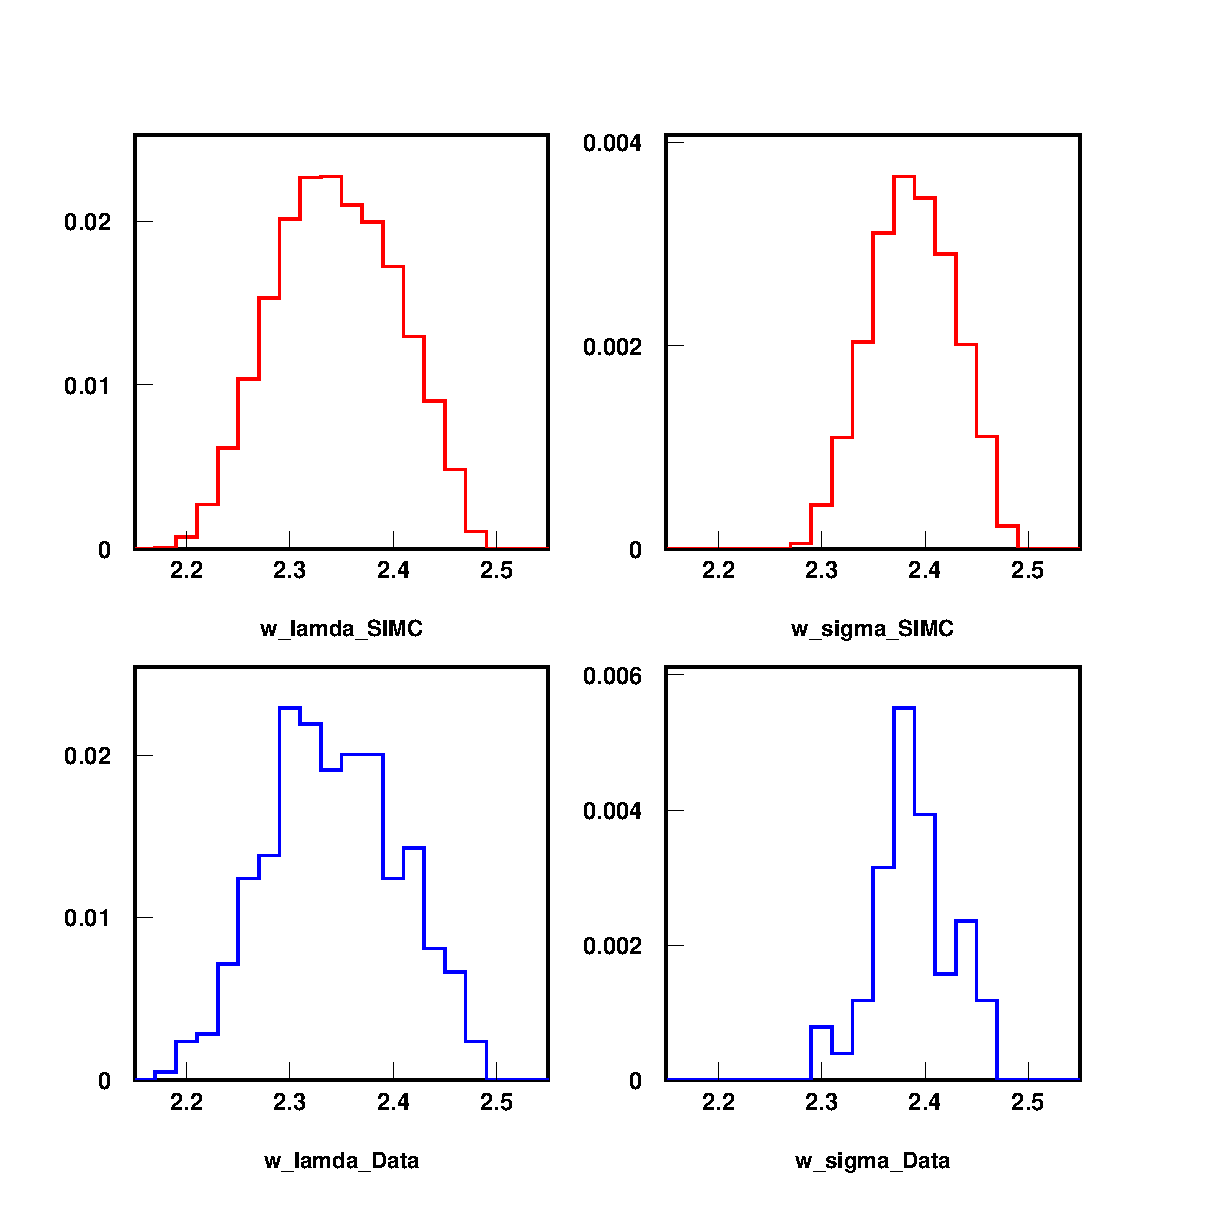
\includegraphics[width=0.8\columnwidth]{com_plot_w_2}
  \caption[Comparison of $W$ from data and SIMC.]{\label{fig:com_plot_w_2}Comparison of $W$ from data and SIMC.\\\\ Clockwise from top left corner: $W_\Lambda$ and $W_\Sigma$ SIMC in RED, $W_\Sigma$ and $W_\Lambda$ data in BLUE for $Q^2$=2.2 $(\mathrm{GeV/c})^2$.}
\end{figure}
%\setlength{\figwidth}{0.8\linewidth}
%\Figure{com_plot_w_2}{\figwidth}{$W$. Clockwise from top left corner: $W_\Lambda$ and $W_\Sigma$ SIMC in \textcolor{red}{RED}, $W_\Sigma$ and $W_\Lambda$ data in \textcolor{blue}{BLUE} for $Q^2$=2.2 $(\mathrm{GeV/c})^2$.}

\begin{figure}[!tbp]
  \centering
  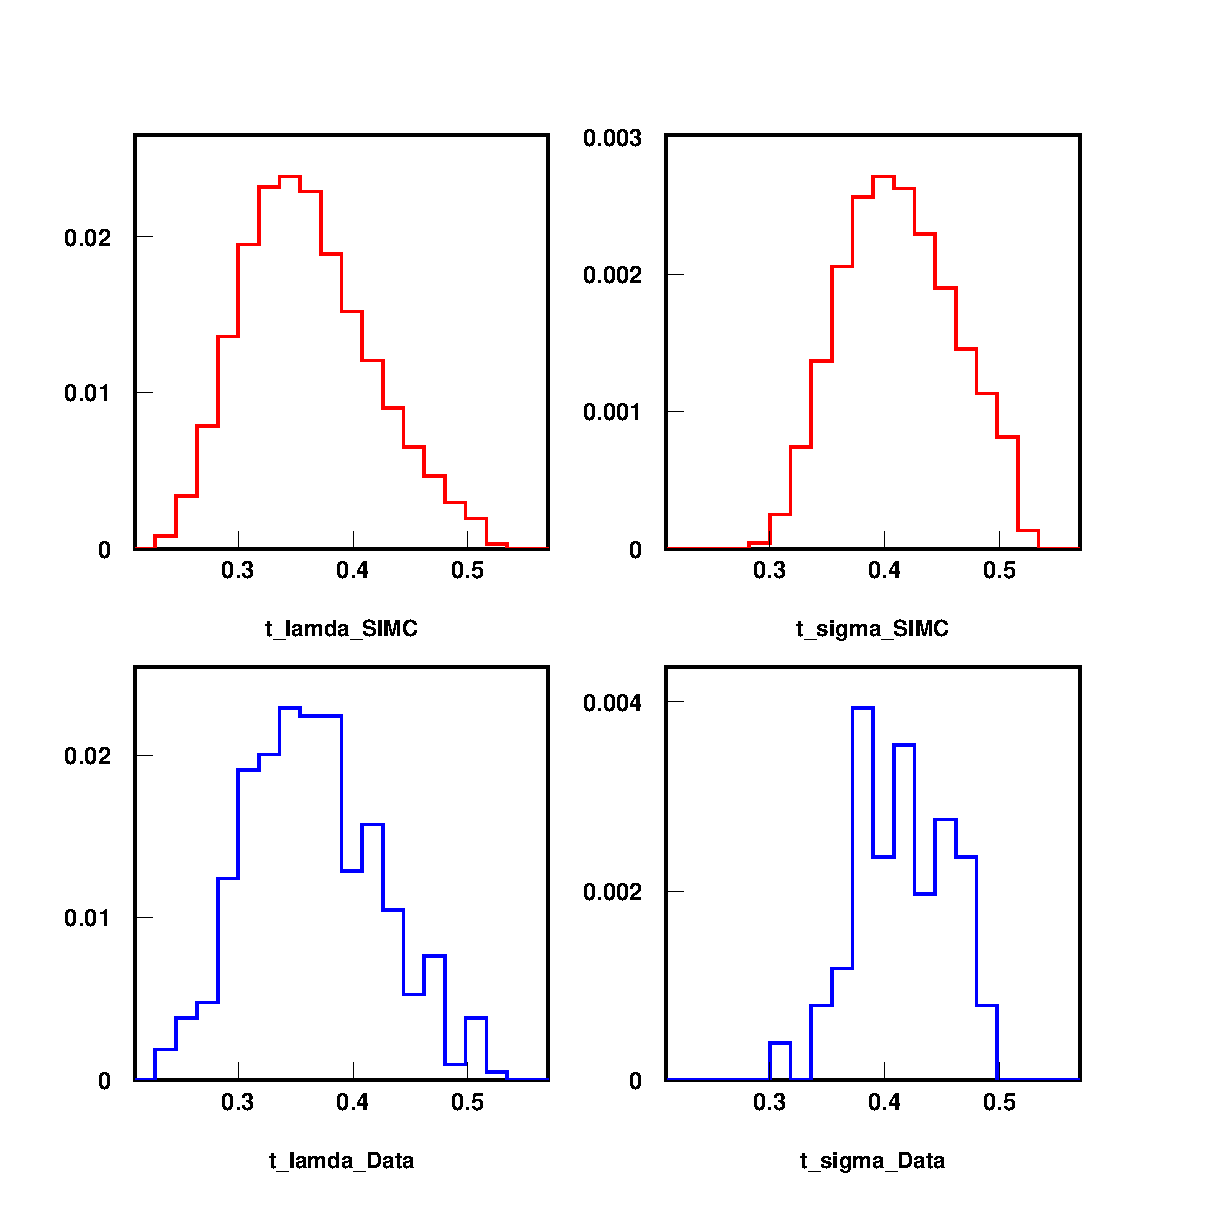
\includegraphics[width=0.8\columnwidth]{com_plot_t_2}
  \caption[Comparison of $t$ from data and SIMC.]{\label{fig:com_plot_t_2}Comparison of $t$ from data and SIMC.\\\\ Clockwise from top left corner: $t_\Lambda$ and $t_\Sigma$ SIMC in RED, $t_\Sigma$ data and $t_\Lambda$ data in BLUE for $Q^2$=2.2 $(\mathrm{GeV/c})^2$.}
\end{figure}
%\setlength{\figwidth}{0.8\linewidth}
%\Figure{com_plot_t_2}{\figwidth}{$t$. Clockwise from top left corner: $t_\Lambda$ and $t_\Sigma$ SIMC in \textcolor{red}{RED}, $t_\Sigma$ data and $t_\Lambda$ data in \textcolor{blue}{BLUE} for $Q^2$=2.2 $(\mathrm{GeV/c})^2$.}

\begin{figure}[!tbp]
  \centering
  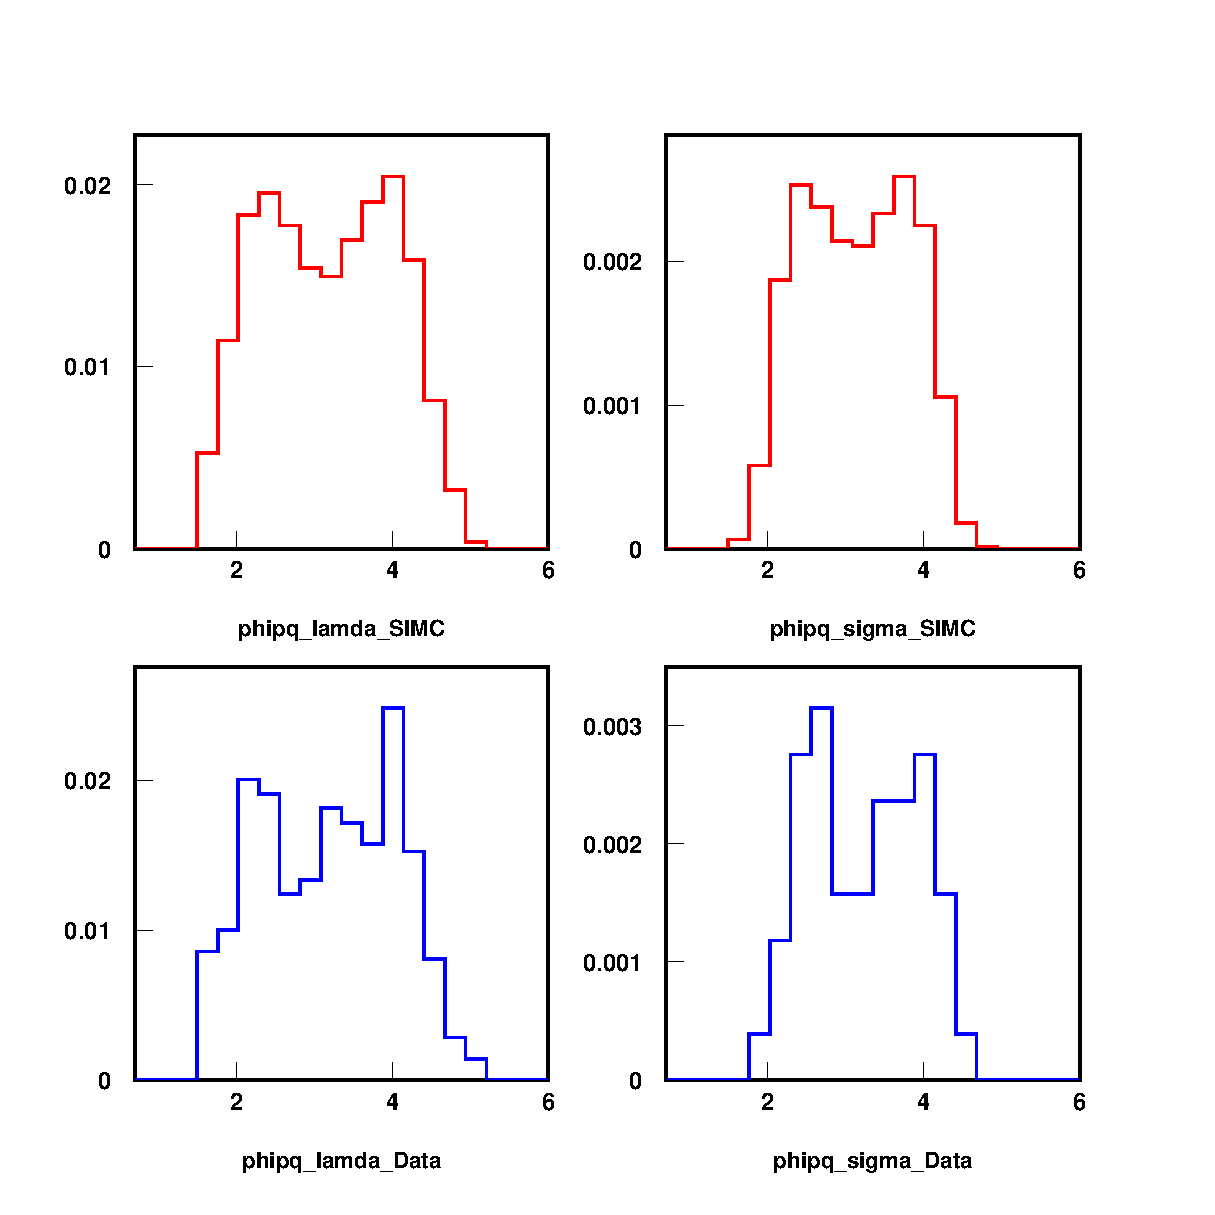
\includegraphics[width=0.8\columnwidth]{com_plot_phi_2}
  \caption[Comparison of $\phi^{pq}$ from data and SIMC.]{\label{fig:com_plot_phi_2}Comparison of $\phi^{pq}$ from data and SIMC.\\\\ Clockwise from top left corner: $\phi^{pq}_\Lambda$ and $\phi^{pq}_\Sigma$ SIMC shown in RED, $\phi^{pq}_\Sigma$ data and $\phi^{pq}_\Lambda$ data in BLUE for $Q^2$=2.2 $(\mathrm{GeV/c})^2$.}
\end{figure}
%\setlength{\figwidth}{0.8\linewidth}
%\Figure{com_plot_phi_2}{\figwidth}{$\phi^{pq}$. Clockwise from top left corner: $\phi^{pq}_\Lambda$ and $\phi^{pq}_\Sigma$ SIMC shown in \textcolor{red}{RED}, $\phi^{pq}_\Sigma$ data and $\phi^{pq}_\Lambda$ data in \textcolor{blue}{BLUE} for $Q^2$=2.2 $(\mathrm{GeV/c})^2$.}

\Section{Iteration}
We have done the iteration on the data to verify our transparency results. As the statistics was very low, we did not expect a large variation in the results. We fitted data for the variables $Q^2$, $W$ and t for $\Lambda$ and $\Sigma$ production as shown in \figureref{fitfunction_kin2_1}, \figureref{fitfunction_kin2_2} and \figureref{fitfunction_kin2_3}, respectively. These fit functions were used to generate the SIMC ntuples. New ntuples were used again for extraction of transparency to check the stability of the yields. This process was repeated doing a second iteration. After the iteration, we did not get any reasonable change in the yields and hence results presented in this thesis are without considering any iteration.

\begin{figure}[!tbp]
  \centering
  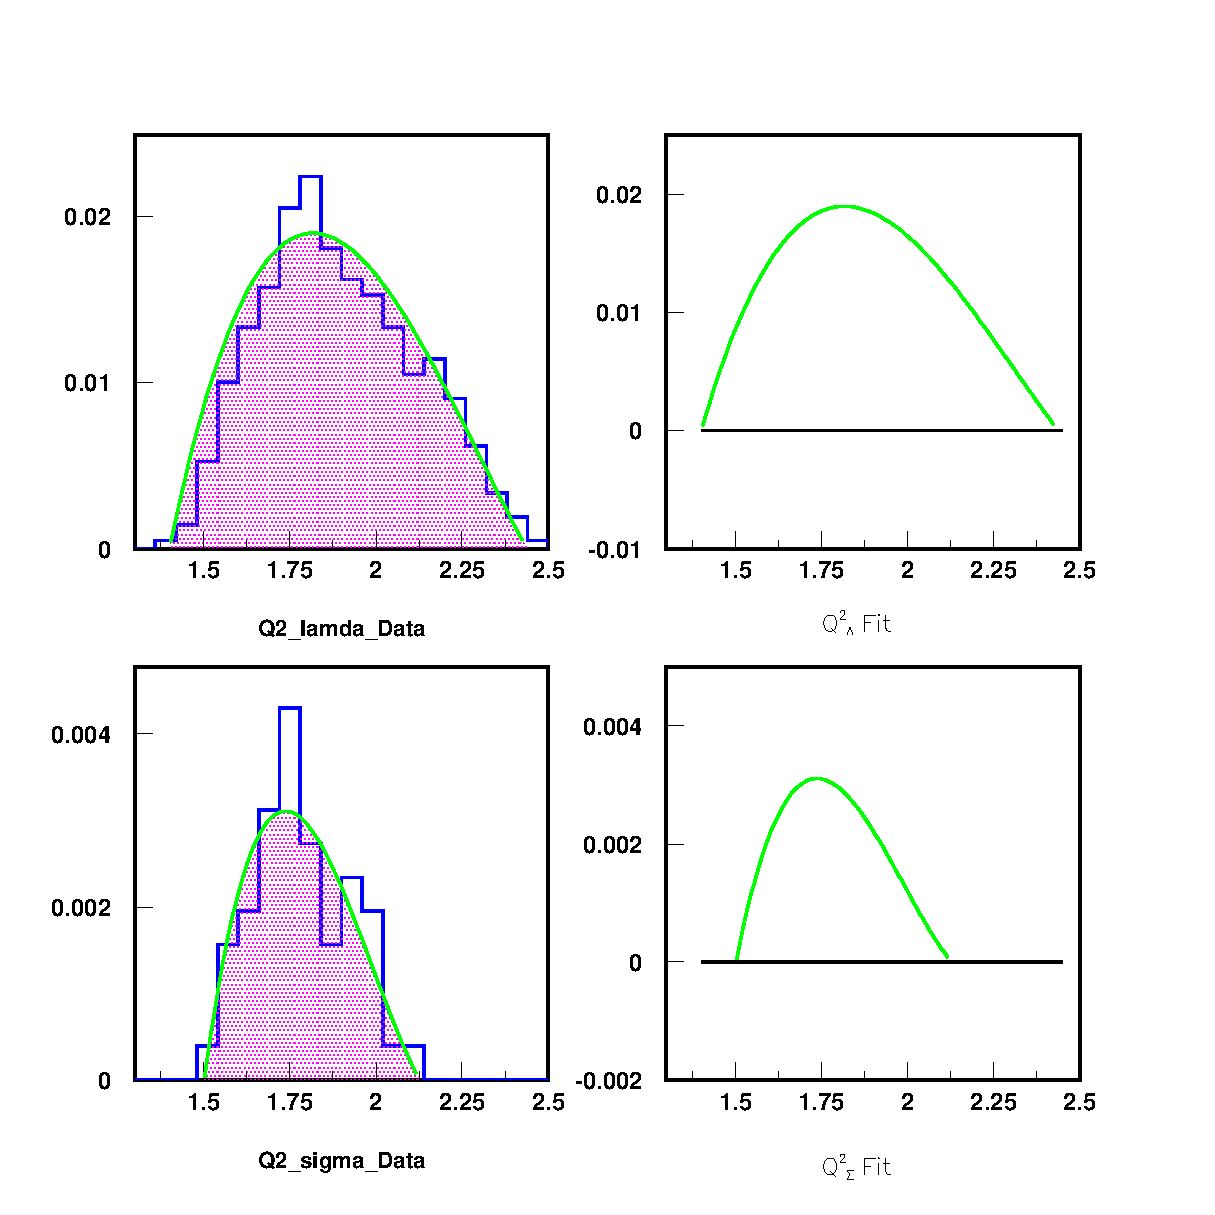
\includegraphics[width=0.8\columnwidth]{fitfunction_kin2_1}
  \caption[Fitting $Q^2$ for iteration.]{\label{fig:fitfunction_kin2_1}Fitting the $Q^2$ data for kinematic settings of $Q^2$=2.2 $(\mathrm{GeV/c})^2$ for iteration.}
\end{figure}
%\setlength{\figwidth}{0.8\linewidth}
%\Figure{fitfunction_kin2_1}{\figwidth}{Fitting the $Q^2$ data for kinematic settings of $Q^2$=2.2 $(\mathrm{GeV/c})^2$ for iteration.}

\begin{figure}[!tbp]
  \centering
  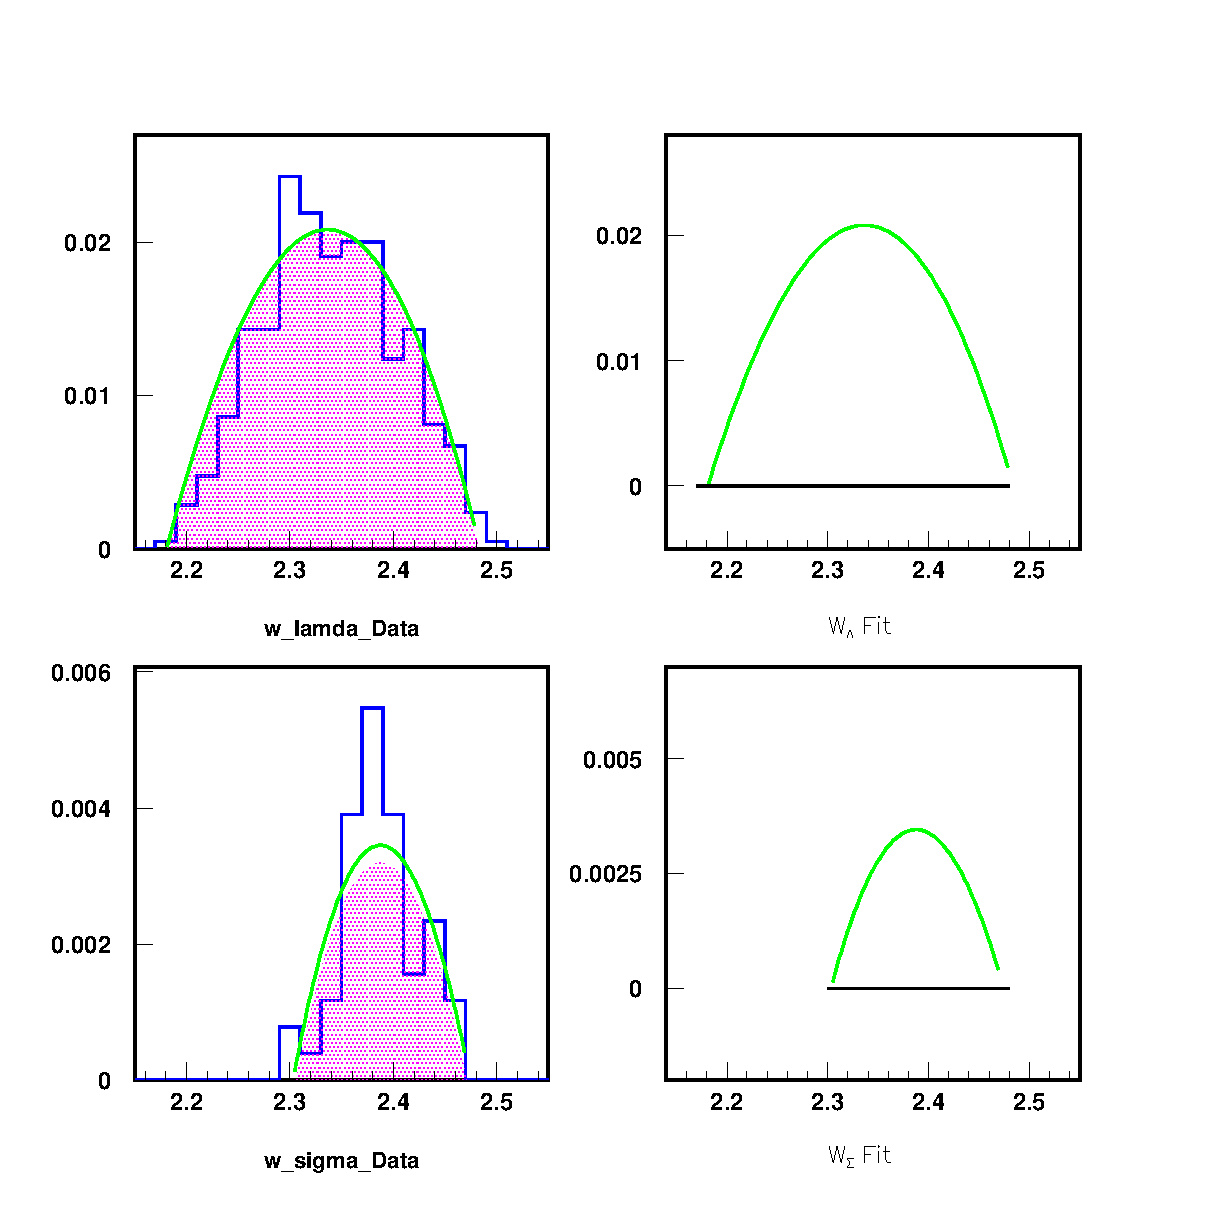
\includegraphics[width=0.8\columnwidth]{fitfunction_kin2_2}
  \caption[Fitting $W$ for iteration.]{\label{fig:fitfunction_kin2_2}Fitting the $W$ data for kinematic settings of $Q^2$=2.2 $(\mathrm{GeV/c})^2$ for iteration.}
\end{figure}
%\setlength{\figwidth}{0.8\linewidth}
%\Figure{fitfunction_kin2_2}{\figwidth}{Fitting the W data for kinematic settings of $Q^2$=2.2 $(\mathrm{GeV/c})^2$ for iteration.}

\begin{figure}[!tbp]
  \centering
  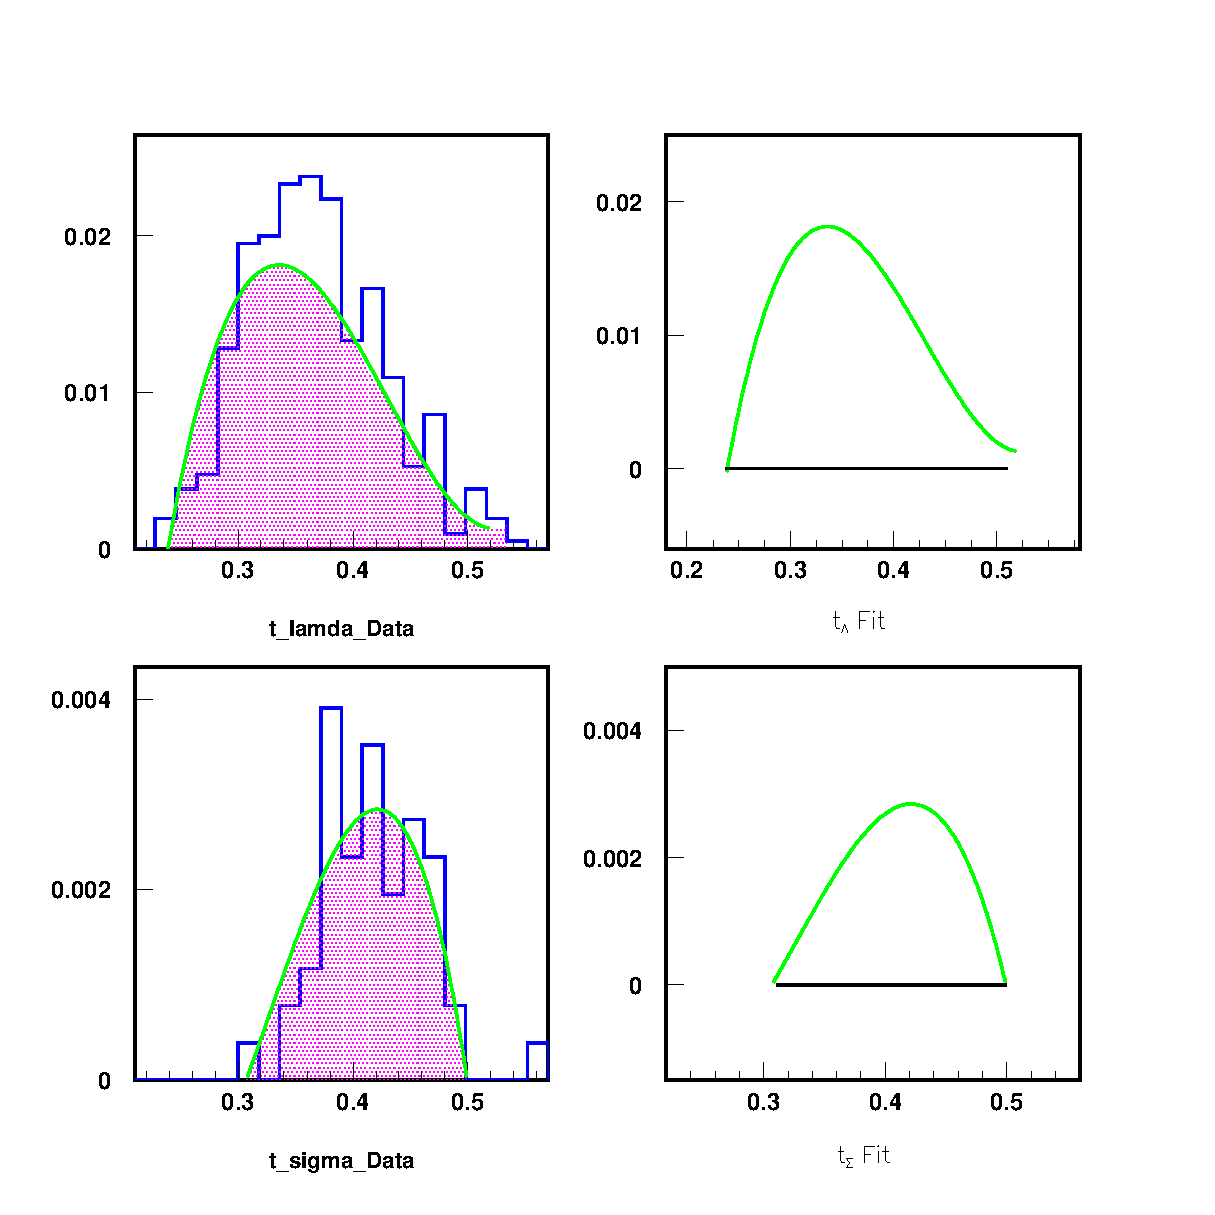
\includegraphics[width=0.8\columnwidth]{fitfunction_kin2_3}
  \caption[Fitting $t$ for iteration.]{\label{fig:fitfunction_kin2_3}Fitting the $t$ data for kinematic settings of $Q^2$=2.2 $(\mathrm{GeV/c})^2$ for iteration.}
\end{figure}
%\setlength{\figwidth}{0.8\linewidth}
%\Figure{fitfunction_kin2_3}{\figwidth}{Fitting the $t$ data for kinematic settings of $Q^2$=2.2 $(\mathrm{GeV/c})^2$ for iteration.}